\chapter{Explorative Datenanalyse}
Das Wichtigste für die künstliche Intelligenz sind die Daten. Beim Erheben der Daten für die künstliche Intelligenz sollten die Datensätze nicht aus kontrollierten Umgebungen stammen die mit festgelegten Rahmenbedingungen arbeiten. Sonst können die Algorithmen unter realen Bedingungen schlecht abschneiden, da hier andere Daten von den Trainingsdaten zu stark abweichen. Daher sollten bereist vorhandenen realen Daten verwendet werden. Daher sind die Modelle mit bereits vorhandenen realen Daten zu trainieren.\vspace{0.2cm}

Die explorative Datenanalyse (\Gls{eda}) wird verwendet, um Daten zu analysieren und ihre Merkmale zusammenzufassen und um besseres Verständnis für die Datensätze zu bekommen. Dies hilft dabei, um herauszufinden wie die Daten am besten verarbeitet werden können. Dabei hilft die \Gls{eda} Muster oder Fehler und Anomalien zu finden, sowie Hypothesen testen und Annahmen zu überprüfen.\vspace{0.2cm}

Sind die Daten analysiert können sie mithilfe, beispielsweise von maschinelles Lernen verarbeitet werden.

\section{Arten der EDA}
Primär unterschiedet [\href{https://www.ibm.com/de-de/cloud/learn/exploratory-data-analysis}{ibm.com}] vier Arten der \Gls{eda}.\vspace{0.2cm}

\textbf{Univariat, nicht-grafisch}\\
Untersucht nur eine Variable und ist somit die einfachste Form der Datenanalyse. Hierbei geht es nicht um Ursachen Forschung oder Finden von Beziehungen, sondern das Beschreiben der Daten und Muster zu finden.\vspace{0.2cm}

\textbf{Univariat, grafisch}\\
In dieser Art gibt es beispielsweise die Möglichkeit eine Variable beispielsweise in einem
\begin{itemize}
	\item Stamm-Blatt-Kurvendiagramm\footnote{Stamm-Blatt-Kurvendiagramm zeigt die alle Datenwerte und die Form der Verteilung.},
	\item Histogramm\footnote{Histogramm mit Balken wird die Häufigkeit oder Anteil der Fälle für einen Wertebereich angezeigt.} oder
	\item Box-Diagramm\footnote{Box-Diagramm fünfstellige Zusammenfassung von 1. Minimum, 2. erstes Quartils, 3. Median, 4. dritten Quartils, 5. Maximum.} dargestellt.
\end{itemize}

\textbf{Multivariat, nicht-grafisch}\\
Diese Daten bestehen aus mehreren Variablen. Sie zeigen allgemeine Beziehungen zwischen zwei oder mehreren Variablen durch Kreuztabellen oder Statistiken.\vspace{0.2cm}
 
\textbf{Multivariat, grafisch}\\
Zeigen grafisch die Beziehungen zwischen ein oder mehreren Variablen. Häufig werden zur Darstellung Streu-\footnote{Streudiagramm, stellen Datenpunkte auf einer horizontalen und einer vertikalen Achse, die Abhängigkeit einer Variablen zu einer anderen zu zeigen.}, Lauf-\footnote{Laufdiagramm ist ein Liniendiagramm von Daten die über die Zeit aufgetragen werden.}, Blasendiagramme\footnote{Blasendiagramm ist eine Datenvisualisierung mittels Kreisen.}, Multivariate Diagramme\footnote{Multivariate Diagramm ist eine grafische Darstellung zwischen Faktoren und einer Antwort.} und Heat-Maps\footnote{Heat-Map hierbei werden die Daten durch Farben dargestellt.} verwendet.

%\section{Methoden der Datenanalyse}

\section{Kundengruppen}
Die Kundengruppe muss aus einer homogenen Menge an Kunden bestehen, die gleich Arttribute besitzen. Neben der Unterteilung der Kundengruppen nach dem DiSG Modells werden die Kunden nach ihrer Vorlieben an Artikeln eingeteilt.

\subsection{DiSG Modell}
Das DiSG Modell beschreibt die vier Grundtypen von Persönlichkeiten der Nutzer. Diese sind \textbf{D}ominant, \textbf{i}nitiativ, \textbf{S}tetig und \textbf{G}ewissenhaft. Jeder der vier Grundtypen weist beim Besuch eines Onlineshops andere Verhaltensmuster auf.\vspace{0.2cm}

Die Grundlagen für dieses Modell beruhen auf der Arbeit von William Moulton Marston aus dem Jahr 1928.

\begin{figure}[!ht]
	\centering
	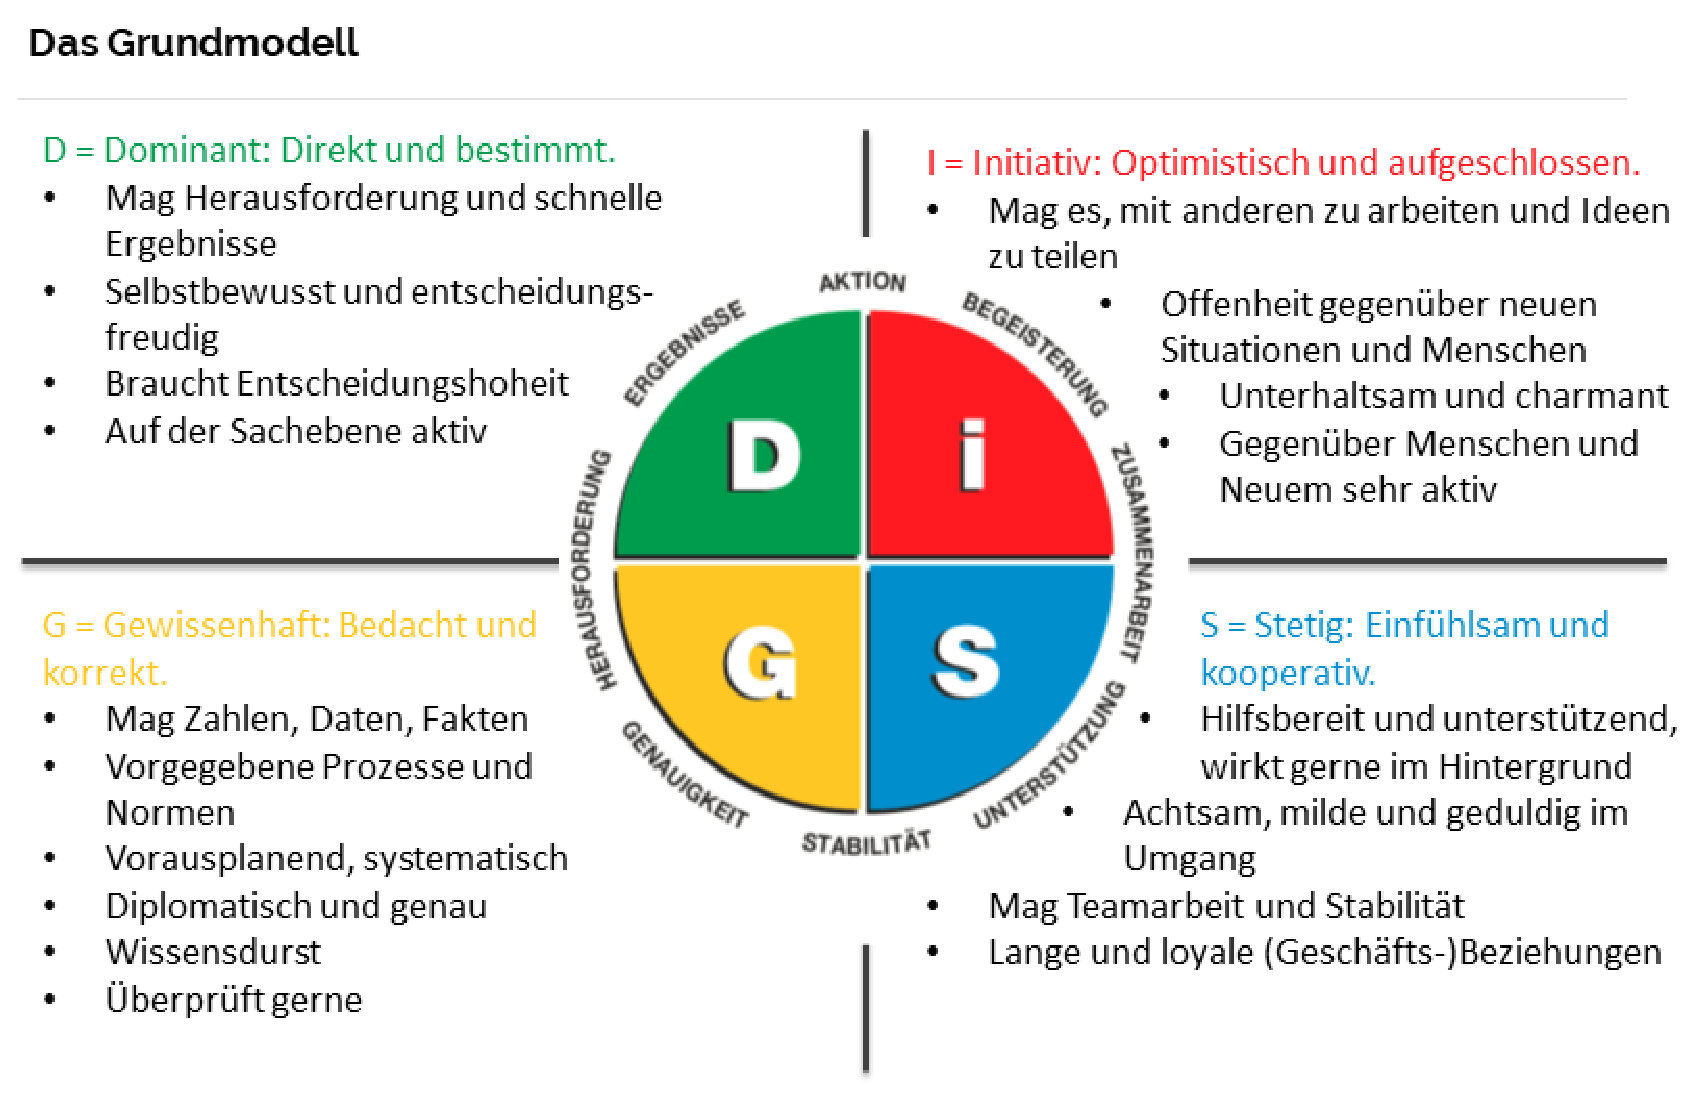
\includegraphics[width=\linewidth]{images/chapter3/disg-uebersicht.eps}
	\caption{DiSG Übersicht \href{https://www.disg-modell.de/persoenlichkeitsorientiertes-lernen-mit-dem-disg-modell}{https://www.disg-modell.de}}
	\label{img:disg_overview}
\end{figure}

Der \textit{Dominante}, hat konkrete Erwartungen an ein Produkt. Daher sollte eine Produktbeschreibung nicht nur klar und deutlich sein, sonder ebenso dessen Nutzen, welche Funktionen es hat, warum es so gut funktioniert und die wie es die Probleme des Kunden löst.\vspace{0.2cm}

Der \textit{Initiative} Kundentyp ist begeisterungsfähig, extrovertiert und optimistisch. Da dieser Typ eher die positiven Eigenschaften eines Produktes sieht, lohnt es sich diesen Kundentyp Rezensionen schreiben zu lassen. Er legt Wert auf eine Wertbeschreibung des Produktes. Dies kann mit \Gls{storytelling} erfolgen.\vspace{0.2cm}

Der \textit{Stetige} kann eine harte Nuss für Onlinehändler sein, da dieser Kundentyp sehr viel Wert auf Produktbeschreibung legt, die dessen Bedürfnisse und Ziele erfasst. Andererseits ändern sich die Bedürfnisse dieses Typs nicht über Nacht. Somit kann er zu einem regelmäßigen kaufenden Stammkunden werden. Die Produktbeschreibung sollte die \Gls{unique_selling_point} enthalten und herausstellen welche Ziele das Produkt, wie unterstützt.\vspace{0.2cm}

Der \textit{Gewissenhafte} geht systematisch vor und analysiert seine Erkenntnisse zum Produkt. Ist eher reserviert und zurückhaltend und schreibt somit weniger Rezensionen. Dieser Typ kann mit Daten und Fakten überzeugt werden. Dies sollte mit Anwendungsbeispielen und Studienergebnissen untermauert werden.

%\subsection{Mögliche Kundengruppen}
%Nach \href{https://www.exali.de/Info-Base/ki-onlineshop}{KI im Onlineshop: So steigern Onlinehändler ihren Umsatz}\vspace{0.2cm}

%Der \textit{Performer} (hat ernste Kaufabsicht und weiß genau was er will) nutzt Suchfunktion und geht gleich in die Kategorie. «Diesem Kunden kann die Suchfunktion besonders angezeigt werden, da er zielstrebig etwas sucht. Findet er es nicht, sucht er auf anderen Seiten weiter.»\vspace{0.2cm}

%Der \textit{Stöberer} (will sich beim stöbern inspirieren lassen) klick auf der Startseite viel herum. «Diesem Kunden könnten Angebote angezeigt werden, die diesem Kunden zum Kauf anregen.»\vspace{0.2cm}

%Nach \href{https://www.businessinsider.de/gruenderszene/allgemein/kundentypen-comarch}{Die 6 häufigsten Kundentypen und wie man sie am besten anspricht}\vspace{0.2cm}

%Der \textit{Schnäppchenjäger} (Hautsache Preiswert) dieser Kunde baut keine richtige Beziehung  zu einem Onlineshop auf. Diese Kunden besuchen meist mehrere Webshops und/oder kommen von Preissuchmaschinen. Diesen Kunden zu binden ist eine Herausforderung. «Dieser Kunde kann effektiv mit Rabatte, Gutscheincodes oder Ausverkaufsaktionen ansprechen. Auch E-Mail-Aktionen lassen sich bei diesem Kundentyp leicht anbringen.»\vspace{0.2cm}

%Der \textit{Eilige} (stehen unter Zeitdruck oder wollen sie sich nicht nehmen) bringt keine Zeit für ein ausgiebiges Shoppingerlebnis mit. Sie verfügen oft über hohe monetäre Mittel, um sich beispielsweise Expresslieferung zu leisten.«Er braucht eine strukturierte Webseite, auf die er Informationen schnell findet. Dies kann durch Suchfunktion für Preis, Größe, usw., eine Schnellansicht für Artikel auf der Übersichtseite mit deutlichem Produktabbildungen.»\vspace{0.2cm}

%Der \textit{Stöberer} (sind Gelegenheitskäufer) schaut stundenlang im Internet ohne bestimmte Absicht. Hierbei ist es schwer vorhersagbar, was dieser Kunde kauft. Oft legt dieser Kunde ein oder zwei Artikel in den Warenkorb, schließt die Bestellung nie ab.«Diese Kunden kennen die Preise im Internet und lassen sich evtl. durch ein Rabattangebot oder Preisnachlass umstimmen.»\vspace{0.2cm}

%Der \textit{Sammler} (auf der Suche nach Besonderheiten) sucht Unikaten oder ganz bestimmte Artikel wie Sondereditionen oder limitierte Ausgaben. Lieferzeiten und Preise spielen keine Rolle. «Bei diesem Kunden sollten Lagerinformationen stets aktuell sein. Ist nach dem Bestellvorgang ersichtlich, dass der Artikel nicht mehr vorhanden ist, wird meist storniert und der Kunde kommt nicht mehr wieder.»\vspace{0.2cm}

%Der \textit{Misstrauische} (Angst Oper zu werden) ziehen große bekannte Onlinehändler vor, da sie befürchten das bei kleineren Probleme auftreten können. Das Misstrauen geht so weit, das dieser Kundentyp nur per Nachname bestellt oder die Ware Selbst abholt. «Dieser Zielgruppe sind Rückgaberecht und Garantieleistungen besonders wichtig. Ebenfalls können diese Kunden durch zusätzliche Versicherungen gewonnen werden.»\vspace{0.2cm}

%Der \textit{Schüchterne} (anonym ist wichtig) kaufen online, da es ihnen peinlich ist, den gesuchten Artikel im stationären Handel zu kaufen. «Diese Kunden nutzen häufig Suchmaschinen und gelangen so in den Shop (SEO ist hier wichtig). Ein weiteres Kriterium für den Schüchternen sind seriöse Bezahl- und Versandarten.»

\section{Daten für die Onlineshop-Nutzeranalyse}
% Hier auch noch etwas über Datenintegration.
Um das Modell zu trainieren kommen bereits erhobene, interne und offene
Daten zu Anwendung. Dabei werden die Daten konsolidiert und deren Integrität geprüft.\vspace{0.2cm}

\textbf{Daten aus dem Shop}\vspace{0.1cm}

Diese Daten sind die ausführlichsten Daten. Sie enthalten unter anderem die Nutzerdaten, Daten zu den ab- und nicht abgeschlossenen Käufen. Dazu gehören u.a. die Höhe der Verkäufe, welche und wie viele Produkte und Zeitpunkt des Kaufabschlusses.\vspace{0.2cm}

\textbf{Daten von Google Analytics}\vspace{0.1cm}

Hier handelt es sich um Nutzerdaten, die deren Verhalten und Bewegung innerhalb der Webseite getrackt wurden.\vspace{0.2cm}

\textbf{interne Daten}\vspace{0.1cm}

Diese Daten werden verwendet, um Zeitpunkte berücksichtigt, bei denen Kunden aktiv mit bestimmten Produkten beworben wurden. Dies soll verhindert das in den Ergebnissen Verzerrungen zu bestimmten Produkten entstehen.\vspace{0.2cm}

\textbf{Offene Daten}\vspace{0.1cm}

Für die Auswertung werden sogenannte ,,Open Data'' verwendet, um saisonale und Feiertage zu berücksichtigen.\vspace{0.2cm}

Aus den gesammelten Daten, die das Nutzer- und Kaufverhalten repräsentieren, soll die Klassifizierung der Nutzer erfolgen. Für die Ermittlung der Klassifizierung wird bei der Berechnung die Daten verwendet, bei denen ein Nutzer einen Kauf abgeschlossen hat. Die folgenden Daten finden Berücksichtigung,
\begin{itemize}
	\item Warenkorbhöhe
	\item Gekauften Artikel pro Warenkorb
	\item Anzahl der zuvor besuchten Seiten
	\item Einstiegsseite
	\item Datum, aus den Open Data
\end{itemize}
Nun erfolgt die Vergleichsberechnung mittel FP-Growth-Algorithmus und eines neuronalen Netzwerks.
